%\documentclass[12pt,a4paper]{report}
\documentclass[12pt,a4paper]{article}

% ---------- Packages ----------
\usepackage[utf8]{inputenc}
\usepackage[T1]{fontenc}
\usepackage{lmodern}
\usepackage{graphicx}
\usepackage{amsmath, amssymb}
\usepackage{geometry}
%\usepackage{hyperref}    % this keeps all colors and boxes
\usepackage{fancyhdr}
\usepackage{setspace}
\usepackage{caption}
\usepackage[numbers]{natbib}  % For bibliography
\usepackage{tocloft} % Custom TOC
\usepackage{url} 
\usepackage{amsthm}
\usepackage[most]{tcolorbox}
\newtheorem{lemma}{Lemma}
\tcbuselibrary{theorems}
\usepackage[hidelinks]{hyperref}  % his removes all colors and boxes 



\newtcbtheorem[auto counter, number within=section]{boxedlemma}{Lemma}%
{colback=blue!5!white, colframe=blue!75!black,
	fonttitle=\bfseries, coltitle=black, boxed title style={colback=white},
	enhanced, attach boxed title to top left={xshift=0.5cm,yshift=-1mm}}%
{lem}





% ---------- Page Setup ----------
\geometry{margin=1in}
\setstretch{1.2}
\pagestyle{fancy}
\fancyhf{}
\rhead{\thepage}
\lhead{Statistical distributions for modeling steel grade compositions}

% ---------- Title ----------
\title{Statistical distributions for modeling steel grade compositions  }
\author{Ehsan Namjoo}   % Print author's name
%\date{\today}

% ---------- Document ----------{\LARGE {\tiny {\small }}}
\begin{document}
	
	\maketitle
	\tableofcontents
	\newpage
	
	
	% ---------- Sections ----------
	\section{Introduction} \label{h:intro}
	In many steel recycling operations, steel scrap is not fully sorted before processing. As a result, a single batch of scrap can contain a mixture of different kind of materials. This variability poses challenges for recycling, especially when high-quality or specialized steel is required. The presence of different alloying elements can significantly affect the properties of the recycled steel. Steel scrap is typically composed of various steel grades and sometimes even non-ferrous metals. Steel grades are classifications used to distinguish different types of steel based on their chemical composition, mechanical properties, and intended applications. These grades are standardized by various national and international organizations to ensure consistency and interoperability across industries.
	To address these challenges, advanced analytical techniques such as Laser-Induced Breakdown Spectroscopy (LIBS), X-ray fluorescence (XRF), and optical emission spectroscopy (OES) are employed. These methods allow recyclers to analyze the elemental composition of scrap quickly and accurately. LIBS, in particular, is valued for its speed and ability to detect multiple elements simultaneously. 
	LIBS is a powerful analytical technique for identifying steel grades and determining the percentage of alloying elements \cite{Legnaioli_LIBS_Metals_2014}. The process involves focusing a high-energy laser pulse on the steel surface, which generates a microplasma. As this plasma cools, it emits light containing spectral lines unique to the elements present in the sample. These spectral signatures are then analyzed to identify and quantify the elemental composition of the steel.
	By identifying the specific steel grades and separating unwanted materials, these techniques help ensure that the recycled steel meets the necessary quality standards. 

 
 
	For steel grade classification, LIBS data can be processed using machine learning models. These models can classify steel types based on their spectral properties \cite{Lin2024}. 	In terms of quantitative analysis, LIBS can determine the concentration of alloying elements. This is typically done using calibration models, where known concentrations are used to train regression algorithms. Studies, such as  \cite{Traparic2023} and  \cite{Jiang2020}, demonstrate the application of machine learning techniques for estimating the elemental composition of alloys.
	
	A well-curated and representative LIBS dataset is fundamental to the success of machine learning models in spectroscopic analysis. The accuracy, robustness, and generalizability of predictive models—whether for classification or quantitative analysis—are directly influenced by the quality and diversity of the training data. A comprehensive dataset should encompass a wide range of sample compositions, experimental conditions, and spectral variations to ensure the model can learn meaningful patterns and avoid overfitting. Without a reliable dataset, even the most sophisticated algorithms may yield poor predictions.
	
	Given the vast number of standardized steel grades, generating a reliable LIBS dataset begins with narrowing the scope to a subset of grades that are most relevant to the intended application (this subset could include the steel grades presented in Deliverable 3.2, Figure 5). Once this subset is defined, the next step involves simulating variations in elemental concentrations within each selected grade to reflect realistic manufacturing and compositional differences. The final stage is to generate LIBS spectra from the elemental compositions provided by the statistical model. This report focuses specifically on the statistical methodologies that can be employed to generate realistic variations in elemental concentrations.
	
	The remainder of this report is organized as follows. Section \ref{h:Probability distributions} provides a brief overview of probability distributions, followed by an introduction to several distributions that may be useful for modeling variations in steel grades. Section \ref{h:Statistical modeling} focuses on practical aspects of generating samples from specific probability density functions. Section \ref{h:Discussion} presents a discussion of the different modeling approaches, and suggest a practical solution, and finally Section \ref{h:Conclusion} provides a summary.

	
	\section{Probability distributions to model steel grades} \label{h:Probability distributions}
	Steel grades are defined by specific characteristics and consist of predefined ranges of alloying elements. For example, Table \ref{table:aisi4042} illustrates the concentration ranges of the constituent elements in the steel grade AISI 4042 \cite{matweb2025}.  
	\begin{table}[h!]
		\centering
		\caption{Chemical composition of AISI 4042 steel}
		\begin{tabular}{|l|c|}
			
			\hline
			\textbf{Element} & \textbf{Composition (\%)} \\ \hline
			Carbon (C)       & 0.40 – 0.45 \\ \hline
			Iron (Fe)        & 97.93 – 98.55 \\ \hline
			Manganese (Mn)   & 0.70 – 0.90 \\ \hline
			Molybdenum (Mo)  & 0.20 – 0.30 \\ \hline
			Phosphorus (P)   & $\leq$ 0.035 \\ \hline
			Silicon (Si)     & 0.15 – 0.35 \\ \hline
			Sulfur (S)       & $\leq$ 0.040 \\ \hline
		\end{tabular}
				\label{table:aisi4042}
	\end{table}	
	Since the concentration of each alloying element in a specific steel grade is defined within a predetermined range, any real sample of that grade may exhibit elemental values anywhere within those limits. To construct a reliable dataset, one can randomly generate concentrations for each element based on an appropriate probability distribution. Naturally, the support of each distribution must align with the predefined range for the corresponding element. Figure \ref{fig:prob_dens} illustrates an hypothetical probability density function for the Silicon concentration in AISI 4042. In the following some probability distribution that might be appropriate to model steel grades are introduced.
	\begin{figure}[h!]
		\centering
		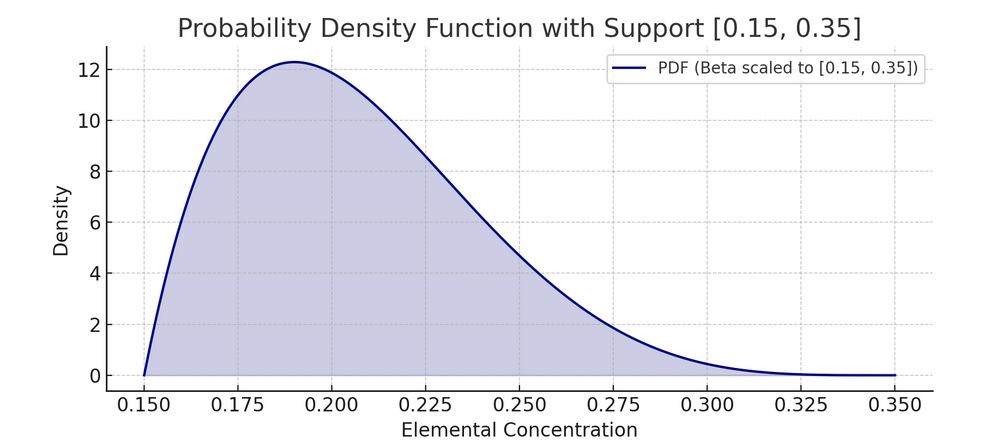
\includegraphics[width=0.7\textwidth]{Prob_dens.png}
		\caption{A hypothetical distribution for Si concentration}
		\label{fig:prob_dens}
	\end{figure}
	\subsection{Gaussian distribution}
	The Gaussian distribution, also known as the normal distribution, is a continuous probability distribution that plays a central role in statistics and machine learning. It is characterized by its symmetric, bell-shaped curve, which is defined by two parameters: the mean ($\mu$), indicating the center of the distribution, and the standard deviation ($\sigma$), which measures the spread of the data around the mean. The Gaussian distribution is often observed in natural phenomena and is widely used for modeling measurement errors, data noise, and as an underlying assumption in many statistical models. Equation~\ref{eq:gaussian_pdf} shows the probability density function of the Gaussian distribution.
	\begin{equation}
		f(x) = \frac{1}{\sqrt{2\pi\sigma^2}} \, \exp\left( -\frac{(x - \mu)^2}{2\sigma^2} \right)
		\label{eq:gaussian_pdf}
	\end{equation} 
	\subsection{Gamma distribution} \label{h:Gamma distribution}
	The Gamma distribution is a continuous, asymmetric probability distribution that is defined for positive real numbers, unlike the Gaussian distribution which spans the entire real line. Equation \ref{eq:gamma_pdf} presents the probability density function of the Gamma distribution.
	\begin{equation}
		f(x; \alpha, \theta) = \frac{\theta^\alpha}{\Gamma(\alpha)} x^{\alpha - 1} e^{-\theta x}, \quad x > 0
		\label{eq:gamma_pdf}
	\end{equation}
	$\alpha$ and $\theta$ are shape and scale parameters respectively. The Gamma function, denoted as $\Gamma(.)$, is a continuous extension of the factorial function to all complex numbers (except for non-positive integers). It is defined by the improper integral:
	\begin{equation}
		\Gamma(\alpha) = \int_0^{\infty} t^{\alpha - 1} e^{-t} \, dt.
		\label{eq:gamma_function}
	\end{equation}
	
	For positive integers, the Gamma function satisfies the identity $\Gamma(n) = (n - 1)!$, which makes it a natural generalization of the factorial. 
	

	\subsection{Beta distribution}
	The Beta distribution is another continuous probability distribution, commonly used to model random variables that take on positive values within a fixed interval. It differs fundamentally from the Gamma distribution described earlier. While the Gamma distribution is defined over the interval $(0,\infty)$, the Beta distribution is limited to the interval $(0,1)$. Like the Gamma distribution, the shape of the Beta distribution is determined by two parameters. It is particularly useful for modeling probabilities or proportions. Although its standard form is confined to $(0, 1)$, the Beta distribution can be easily transformed to cover any arbitrary interval. For example Figure \ref{fig:prob_dens} is basically a Beta distribution that has been mapped to the interval $(0.15,0.35)$.
	The probability density function  of the Beta distribution with shape parameters \( \alpha > 0 \) and \( \beta > 0 \) is given by:
	\begin{equation}
		f(x; \alpha, \beta) = \frac{1}{B(\alpha, \beta)} \, x^{\alpha - 1} (1 - x)^{\beta - 1}, \quad \text{for } x \in (0, 1)
		\label{eq:beta_pdf}
	\end{equation}
	
	Here, \( B(\alpha, \beta) \) is the Beta function, defined as:
	\begin{equation}
		B(\alpha, \beta) = \int_0^1 t^{\alpha - 1} (1 - t)^{\beta - 1} \, dt = \frac{\Gamma(\alpha)\Gamma(\beta)}{\Gamma(\alpha + \beta)}
		\label{eq:beta_function}
	\end{equation}
	


	\subsection{Dirichlet distribution}
	The Dirichlet distribution is a multivariate probability distribution used to model random variables that represent proportions of a whole specifically, a set of positive values that sum to 1. 
    A random vector $\mathbf{X}=(X_1, X_2, \ldots, X_K)$ that follows a Dirichlet distribution is denoted as: 
	\begin{equation}
		\mathbf{X} \sim \operatorname{Dir}(\boldsymbol{\alpha})
	\end{equation}
	
	where 
	
	\begin{equation}
		X_i \geq 0 \quad \text{for all } i \quad \text{and} \quad \sum_{i=1}^K X_i = 1
	\end{equation}
	
	The probability density function of the Dirichlet distribution is given by:
	
	\begin{equation}
		f(x_1, \ldots, x_K; \alpha_1, \ldots, \alpha_K) = 
		\frac{1}{B(\boldsymbol{\alpha})} \prod_{i=1}^K x_i^{\alpha_i - 1}
		\quad \text{for } x_i > 0 \text{ and } \sum_{i=1}^K x_i = 1
		\label{eq:dirichlet_pdf}
	\end{equation}
	
	where, \( B(\boldsymbol{\alpha}) \) is the multivariate Beta function, defined as:
	
	\begin{equation}
		B(\boldsymbol{\alpha}) = \frac{\prod_{i=1}^K \Gamma(\alpha_i)}{\Gamma\left( \sum_{i=1}^K \alpha_i \right)}
		\label{eq:multivariate_beta_function}
	\end{equation}
	and  \( \Gamma(\cdot) \) is the Gamma function defined in subsection \ref{h:Gamma distribution}.
	\noindent
	In the Dirichlet distribution, the vector of parameters is called the \textit{concentration vector}, typically denoted by
	\[
	\boldsymbol{\alpha} = (\alpha_1, \alpha_2, \dots, \alpha_K),
	\]
	where each component satisfies \( \alpha_i > 0 \). The concentration vector determines the shape of the distribution over the probability simplex.
	
	The probability simplex is the geometric space that represents all possible sets of probabilities for a finite number of categories. More precisely, it is the set of all vectors whose components are non-negative and sum to one.
	
	Formally, for a discrete probability distribution over \(K\) categories, the  probability simplex \(\Delta^{K-1}\) is defined as
	\[
	\Delta^{K-1} = \left\{ (x_1, x_2, \ldots, x_K) \in \mathbb{R}^K \; : \; x_i \geq 0, \quad \sum_{i=1}^K x_i = 1 \right\}.
	\]
	Since the components sum to one, the simplex is a \((K-1)\)-dimensional subset embedded in \(\mathbb{R}^K\).
	
	Intuitively, for \(K=2\), the simplex \(\Delta^1\) corresponds to the line segment between the points \((1,0)\) and \((0,1)\) in $\mathbb{R}^2$. Each point on this line represents a pair of probabilities summing to one. For \(K=3\), the simplex \(\Delta^2\) is a triangle in three-dimensional space, where each vertex corresponds to one category having probability one and the others zero. Points inside this triangle represent probability triples summing to one. 
	Each \( \alpha_i \) controls the expected weight and concentration of the corresponding component \( X_i \) in the probability simplex.
	An interactive chart that visualizes the Dirichlet distribution in \(\Delta^2\) is available in \cite{dirichlet_plot}. 	 
	When the number of dimensions is \( K = 2 \), the Dirichlet distribution reduces to the Beta distribution. Specifically, the two-parameter Beta distribution is equivalent to the two-dimensional Dirichlet distribution:
	\begin{equation}
	\operatorname{Beta}(\alpha_1, \alpha_2) \equiv \operatorname{Dir}(\alpha_1, \alpha_2).
	\label{eq:beta-dirichlet}
	\end{equation}


	Each component \( X_i \) is marginally distributed according to a Beta distribution:
	\begin{equation}
		X_i \sim \operatorname{Beta}\left( \alpha_i, \sum_{j \ne i} \alpha_j \right).
		\label{eq:dirichlet-marginal}
	\end{equation}

	The expected value of each component \( X_i \) is given by
	\begin{equation}
		\mathbb{E}[X_i] = \frac{\alpha_i}{\sum_{j=1}^K \alpha_j},
		\label{eq:dirichlet-mean}
	\end{equation}
	where the denominator is often denoted by the total concentration parameter \( \alpha_0 \), i.e.,
	\begin{equation}
		\alpha_0 = \sum_{j=1}^K \alpha_j.
		\label{eq:alpha0}
	\end{equation}

	The variance of \( X_i \) is
	\begin{equation}
	\operatorname{Var}(X_i) = \frac{\alpha_i (\alpha_0 - \alpha_i)}{\alpha_0^2 (\alpha_0 + 1)},
	\label{eq:dirichlet-var}
	\end{equation}
	and the covariance between two distinct components \( X_i \) and \( X_j \), for \( i \ne j \), is
	\begin{equation}
		\operatorname{Cov}(X_i, X_j) = -\frac{\alpha_i \alpha_j}{\alpha_0^2 (\alpha_0 + 1)}.
		\label{eq:dirichlet-cov}
	\end{equation}
	Figure~\ref{fig:dirich3d} shows the Dirichlet distribution for different \( \boldsymbol{\alpha} \) vectors for \( K = 3 \). In this case, the Dirichlet distribution is defined on the 2-dimensional simplex.
	
	\begin{figure}[h!]
		\centering
		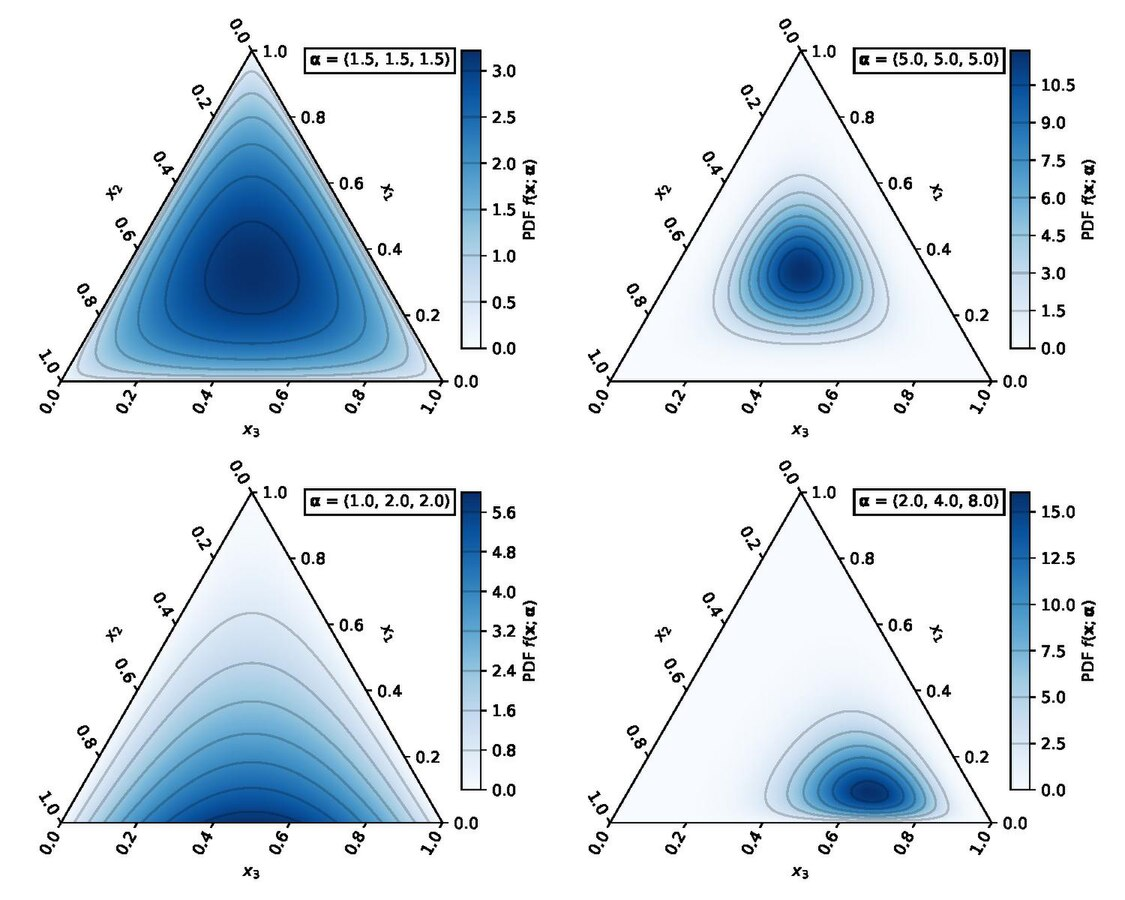
\includegraphics[width=0.7\textwidth]{dirichletDist3d.jpg}
		\caption{Dirichlet distribution for \( K = 3 \) and different \( \boldsymbol{\alpha} \) vectors\cite{wikipedia_dirichlet_pdf}}
		\label{fig:dirich3d}
	\end{figure}
	\subsubsection*{Generating Dirichlet distributed samples}
	\addcontentsline{toc}{subsubsection}{Generating Dirichlet distributed samples}
	\noindent
	The total concentration parameter, $\alpha_0$, 
	controls the overall dispersion of the Dirichlet distribution. When \( \alpha_0 \gg 1 \), the distribution is highly concentrated around its mean, and the samples tend to be tightly clustered with low variance. In contrast, if \( \alpha_0 \ll 1 \), the distribution is sparse, and the samples are typically located near the corners of the simplex, meaning one component is close to 1 while the others are near 0. A special case occurs when \( \alpha_0 = K \) and \( \alpha_i = 1 \) for all \( i \); in this scenario, the Dirichlet distribution becomes uniform over the simplex.
	
	Moreover, the relative values of the individual concentration parameters \( \alpha_i \) affect the shape of the distribution. If some \( \alpha_i \) is much larger than the others, then the corresponding component \( X_i \) will dominate in most samples. The distribution is thus skewed in favor of categories with larger concentration values. For example, if $\alpha = (5, 1, 1)$, 	most samples will have larger $x_1$, while the remaining components will tend to be smaller. On the other hand, if \(
	\boldsymbol{\alpha} = (0.2, 0.2, 0.2),\)
	the samples will lie near the vertices of the simplex, with one component close to 1 and the others close to 0. This behavior reflects the high variability and sparsity of the distribution when the concentration parameters are all less than 1. 
	\noindent
	In such cases, most draws have one dominant component close to 1, while the others are near 0. This effect is amplified when \( \alpha_0 = \sum_{i=1}^K \alpha_i < 1 \), resulting in a high probability density near the edges and vertices of the simplex.
	
	In the case of unequal small concentration parameters, like \(	
	\boldsymbol{\alpha} = (0.3, 0.2, 0.5),
	\)
	the distribution still favors sparsity, but not symmetrically. The component with the highest \( \alpha_i \) (here, \( x_3 \)) is more likely to dominate, but it's still possible for other components to take on large values in individual samples. 
	
	In practice, the Gamma distribution is used to generate Dirichlet distributed samples. The following lemma provide the relevant mathematical background:
% This is in text mode
	\begin{tcolorbox}[colback=gray!10, colframe=black, title=Dirichlet distribution via normalized Gamma variables]
		\begin{lemma}[]
		
			Let \( Y_1, \dots, Y_K \) be independent random variables such that
			\[
			Y_i \sim \mathrm{Gamma}(\alpha_i, 1), \quad \text{for } i = 1, \dots, K,
			\]
			and 
			\[
			X_i = \frac{Y_i}{\sum_{j=1}^K Y_j}.
			\]
			Then \( (X_1, \dots, X_K) \sim \mathrm{Dir}(\alpha_1, \dots, \alpha_K) \).
		\end{lemma}
	\end{tcolorbox}

	According to this lemma, sampling from the Dirichlet distribution is straightforward. One simply generates independent positive real numbers from Gamma distributions and then normalizes them by dividing each value by the total sum. This normalization yields a multivariate vector that follows the Dirichlet distribution.
	
	
	 
	\section{Statistical modeling of steel grade component concentration} \label{h:Statistical modeling}
	In this section, the potential of using the previously introduced probability distributions to model elemental concentrations in steel grades is examined.
 	While numerous well-known distributions could be applied in this context, only a subset was presented in Section~\ref{h:Probability distributions}, each belonging to a distinct family of probability density functions. In the following, each family is first considered in general terms, and the specific distribution introduced in Section~\ref{h:Probability distributions} is then discussed as a representative example for modeling elemental concentrations in steel grades. Finally, the Dirichlet distribution is explored as a candidate for simultaneously modeling all elemental concentrations within a single steel grade, and the necessary conditions on its parameters are presented to support this application.
 	
	
	
	  
	\subsection{Modeling using real-line and one-sided distribution}
	Real-line distributions and one-sided distributions differ primarily in the range of values over which they are defined. Real-line distributions have support over the entire real number line, \( (-\infty, +\infty) \), allowing them to model phenomena that can take both positive and negative values. Common examples include the Gaussian, Cauchy, and Laplace distributions. These are typically symmetric and suitable for modeling deviations around a central value. In contrast, one-sided distributions are defined only over a semi-infinite interval, usually \( [0, \infty) \), making them appropriate for modeling quantities that cannot be negative, such as time, length, or concentrations. Examples include the exponential, gamma, and chi-squared distributions. This distinction in support influences both the mathematical properties and practical applications of these distributions in statistical modeling.
	
	Gaussian and Gamma distributions were introduced as examples of real-line and one-sided distribution  families, respectively, in previous section. Compared to the Gaussian distribution, the gamma distribution is defined only for positive values, making it more suitable for modeling quantities such as the concentrations of elements in steel grades, which cannot be negative. In contrast, the Gaussian distribution assigns non-zero probabilities to negative values, which may be unrealistic in such contexts. While it is possible to reduce the probability of negative values by carefully selecting the mean and variance of a Gaussian distribution, one-sided distributions like the gamma distribution are generally preferred, as they provide a more realistic representation of inherently non-negative data. Furthermore, the Gamma distribution is inherently flexible in modeling skewed data due to its shape parameter, whereas the Gaussian distribution is symmetric by definition. This flexibility makes the gamma distribution particularly well-suited for data that exhibit skewness. 

	\subsection{Modeling using bounded-support distribution}
	Bounded-support distributions are distributions whose probability density functions  are nonzero only within a finite interval. This characteristic makes them particularly suitable for modeling elemental concentrations in steel grades, as these concentrations are inherently constrained within specific limits. Unlike unbounded distributions, bounded-support distributions ensure that modeled values remain within realistic ranges, preventing the generation of physically impossible negative concentrations or values exceeding maximum feasible levels. Additionally, these distributions can effectively capture the variability and uncertainty of elemental compositions while respecting natural boundaries, leading to more accurate models. Uniform, Beta, and truncated normal distributions are some examples within this family.
	
	\subsection{Modeling using Dirichlet distributions}
	Since a $K$-dimensional vector drawn from a Dirichlet distribution lies within the $(K\!-\!1)$-dimensional simplex $\Delta^{K-1}$, the Dirichlet distribution offers a natural framework for generating vectors of concentrations that sum to one. In the context of steel grades, such vectors can represent the percentage composition of different elements. However, additional constraints may be necessary to ensure that the generated samples remain within predefined bounds for each individual component. In another words, the parameters of Dirichlet distribution should wisely be determined to meet the statistical properties of each of the elemental concentrations. 
	
	Suppose that $\mu_i$ and $\sigma_i$ represent the mean and variance, respectively, of the $i$-th element in the steel grade. These values can be obtained from industrial catalogs and related sources, such as \cite{matweb2025}. The $i$-th marginal distribution of the Dirichlet distribution, as mentioned in Equation~\ref{eq:dirichlet-marginal}, is a Beta distribution with mean and variance given in Equations~\ref{eq:dirichlet-mean} and \ref{eq:dirichlet-var}. Therefore, the following set of equations must hold:


	\begin{flushleft}
		\begin{equation}
			\left\{
			\begin{array}{l}
				\mu_i = \frac{\alpha_i}{\alpha_0} \\[6pt]
				\sigma_i^2 = \frac{\alpha_i(\alpha_0 - \alpha_i)}{\alpha_0^2 (\alpha_0 + 1)}
			\end{array}
			\right.
			\label{eq:mu_sigma}
		\end{equation}
	\end{flushleft}
	It is clear that:
	\[
	\alpha_i = \mu_i \, \alpha_0.
	\]
	and
	\[
	\sigma_i^2 = \frac{\mu_i \, \alpha_0 \left( \alpha_0 - \mu_i \, \alpha_0 \right)}{\alpha_0^2 \, (\alpha_0 + 1)}
	= \frac{\mu_i \, (1 - \mu_i)}{\alpha_0 + 1}.
	\]

	Hence, for each $i$,
	\begin{equation}
		\alpha_0 = \frac{\mu_i \, (1 - \mu_i)}{\sigma_i^2} - 1. \label{eq:alpha0-formula}
	\end{equation}

	Since $\alpha_0$ is the same for all $i$, the quantities in \eqref{eq:alpha0-formula} must be equal for all $i$, which requires:
	\begin{equation}
		\frac{\mu_1 \, (1 - \mu_1)}{\sigma_1^2}
		= \frac{\mu_2 \, (1 - \mu_2)}{\sigma_2^2}
		= \cdots
		= \frac{\mu_K \, (1 - \mu_K)}{\sigma_K^2}
		\label{eq:dirichlet-consistency}
	\end{equation}


	Then $\alpha_0$ can be computed from any of $(\mu_i,\sigma_i^2)$ pairs using \eqref{eq:alpha0-formula}, and the concentration parameter of each component is calculated by $\alpha_i = \mu_i \, \alpha_0$.
	
	The Dirichlet distribution requires positive $\alpha_0$, thus the following equation should also hold:
		\begin{equation}
		\alpha_0 = \frac{\mu_i \, (1 - \mu_i)}{\sigma_i^2} - 1 > 0 \label{eq:alpha0-formula2}
		\end{equation}
	that requires:
	\begin{equation}
		\sigma_i^2 < \mu_i(\mu_i-1) \label{eq:dirichlet-consistency2}
	\end{equation}
	Figure~\ref{fig:beta-mixture} shows the marginal distributions of the Dirichlet distribution for $\boldsymbol{\alpha} = (4, 10, 6)$. Although the Dirichlet distribution guarantees that the sum of the elements in the random vector $\mathbf{X}$ equals one, it is not always possible to force each marginal to exactly follow the predetermined statistical properties, due to the constraints given in Equation~\ref{eq:dirichlet-consistency}. 

	
		
	\begin{figure}[h!]
		\centering
		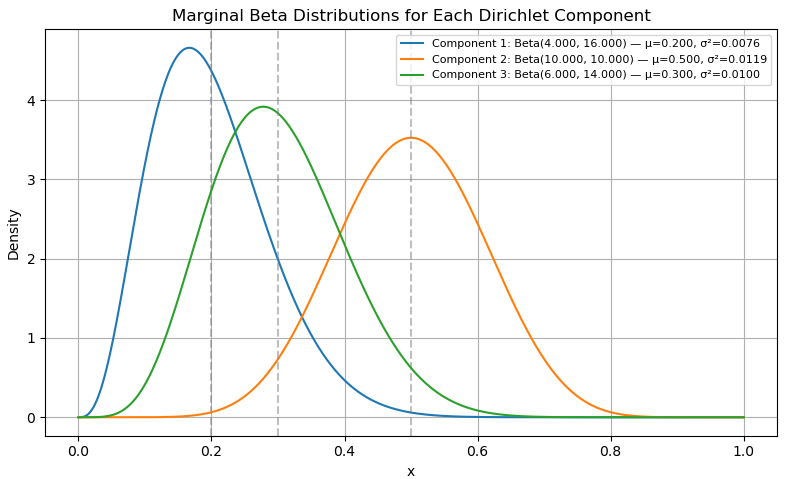
\includegraphics[width=0.7\textwidth]{BetaMixture.png}
		\caption{Marginal Beta distributions for each Dirichlet Component, $\boldsymbol{\alpha}=(4,10,6)$}
		\label{fig:beta-mixture}
	\end{figure}



	
	\section{Discussion} \label{h:Discussion}
	In standard steel grade specifications, it is generally unnecessary to determine the exact weight percentage of iron. This is because iron constitutes the predominant component of steel, and its content is typically reported as the \emph{balance}, the remainder after accounting for all specified alloying elements. Consequently, published chemical compositions in datasheets and standards seldom sum to exactly \(100\%\), with the difference being almost entirely attributable to iron and minor trace elements \cite{huyett_engineering_handbook, nickel_institute_pulp_paper}.

	Moreover, the reported concentrations of alloying elements often follow different formats. For example, according to Table~\ref{table:aisi4042}, the concentration of carbon is specified as a range (from \(0.40\%\) to \(0.45\%\)), while other elements may be given only with an upper limit. This variation makes it challenging to construct a single statistical model that can simultaneously account for all concentration statistics and their respective predefined range.

	In practice, it is not necessary to generate all concentrations simultaneously, since the iron content is always determined by balance. Instead, each alloying element can be modeled individually, and after determining all specified alloying element percentages, the iron content can be calculated by subtracting the sum of these percentages from \(100\%\). In this approach, there is no need to apply multivariate statistical distributions such as the Dirichlet distribution to generate the concentrations of elements in steel grades. 

	Furthermore, aside from the issue of differing predefined ranges for each element, the marginal distributions of a Dirichlet distribution are Beta distributions, which impose constraints on the allowed means and variances of the concentrations, as shown by the equations in \ref{eq:dirichlet-consistency}. Even if meeting these consistency requirements is not strictly impossible, it is often very difficult to find parameters that satisfy all the means and variances in \ref{eq:dirichlet-consistency}. Attempting to do so may also force changes to mean and variance values that are not feasible or practical.

	An alternative approach for generating the percentages is to model each concentration independently using a statistical distribution suited to that element’s predefined range. Bounded-support distributions, such as truncated Gaussian, Beta, or uniform distributions can serve as suitable choices. Once all alloying element concentrations are generated, the iron percentage can then be determined as described earlier.
 

	
\section{Conclusion} \label{h:Conclusion}
Accurately modeling the elemental composition of steel grades is essential for generating realistic datasets, particularly in applications such as LIBS-based analysis and machine learning classification. This report reviewed several statistical distributions for simulating alloying element concentrations, including real-line, one-sided, and bounded-support probability distributions, as well as the multivariate Dirichlet distribution. 

While the Dirichlet distribution offers a theoretically appealing framework for generating vectors of concentrations that sum to unity, its practical application is limited by strict consistency conditions on the means and variances of the marginal distributions. These constraints, together with the diversity in reporting formats and predefined ranges for different alloying elements, make it difficult to fit a  Dirichlet model to real-world steel grade specifications.

Given these challenges, a more flexible and pragmatic approach is to model each alloying element independently, using a bounded-support distribution tailored to its specific compositional range. This method respects individual element constraints, avoids infeasible parameter restrictions, and simplifies the generation process. The iron content can then be computed as the balance, ensuring the total composition sums to \(100\%\). 

This element-wise modeling strategy balances statistical rigor with practical feasibility, enabling the creation of synthetic datasets that are both realistic and aligned with industrial steel grade specifications.

	
	% ---------- References ----------
	\newpage
%	\bibliographystyle{plainnat}
	\bibliographystyle{unsrtnat}
%	\bibliographystyle{abbrvnat}
	\bibliography{references}  % Create a file named references.bib
%	
%	% ---------- Appendix ----------
%	\appendix
%	\chapter{Additional Material}
%	Include supplementary information here.
	
\end{document}
